\documentclass[en,license=none]{../../../eplsummary}

\usepackage{../../../eplcommon}
\usepackage{../../../eplcode}
\usepackage{../../../eplmath}
\usepackage{wrapfig}
\usepackage{float}
\usepackage{multirow}
\usepackage{subcaption}
\lstset{language=Java}

\hypertitle[']{Algorithmics and data structures}{5}{SINF}{1121}
{Charles Momin\and Antoine Paris\and Gilles Peiffer\and Sylvain Ramelot}
{Pierre Schaus}

% TODO
% - improve a lot sections on basic data structures and sorting
% - complete a bit subsection on data compression

\section{Stacks, queues and linked lists}
\begin{mydef}[Linked list]
	A \emph{linked list} is a recursive data structure which is either empty
	(\emph{null}) or a reference to another node containing data and a
	reference to a linked list.
\end{mydef}

In order to define a node, a nested class is used:

\lstinputlisting{code/Node.java}

A linked list allows, with a link to the first and last elements, to realise
the following operations in constant time ($\bigoh(1)$):

\begin{itemize}
	\item inserting at the beginning;
	\item removing an element at the beginning;
	\item inserting an element at the end.
\end{itemize}

In order to randomly insert and remove, one needs to use doubly linked lists
(each node has two links, one in every direction).

The implementations of \lstinline{Stack}, \lstinline{Queue}
and \lstinline{Bag} are based on linked lists. Thanks to these lists, the
required memory space is proportional to the number of items in the collection
and the time required per operation is always independent of the size of the
collection (which wouldn't be the case using arrays for example).

\subsection{Stack}
The working principle of a stack is illustrated in \figuref{stack}.

\begin{figure}[ht]
	\centering
	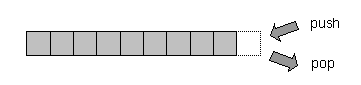
\includegraphics[scale=1.0]{img/stack.png}
	\caption{Illustration of the working principle of a LIFO stack.}
	\label{fig:stack}
\end{figure}

\lstinputlisting{code/Stack.java}

\subsection{Queue}
The working principle of a queue is illustrated in \figuref{queue}.

\begin{figure}[ht]
	\centering
	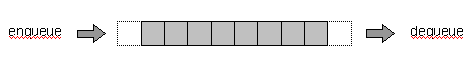
\includegraphics[scale=1.0]{img/queue.png}
	\caption{Illustration of the working principle of a FIFO queue.}
	\label{fig:queue}
\end{figure}

\lstinputlisting{code/Queue.java}

\subsection{Bag}
A bag is simply a stack without a \lstinline{pop()} subroutine.

\section{Sorting algorithms}
The aim of the game here is to sort arrays of items each containing a key
according to a particular order (usually alphabetical or numerical). The notion
of a key is included in a mechanism own to \java{}, the \lstinline{Comparable}
interface (with for example the \lstinline{compareTo} subroutine).

Two types of sorting algorithms exist:
\begin{itemize}
	\item \textbf{in-place} algorithms, which don't (or barely) use additional
	memory;
	\item other sorting algorithms, which need memory to save a copy of the
	array to be sorted in memory.
\end{itemize}

For the sorting algorithms presented in this section, the following template is
used.

\lstinputlisting{code/SortTemplate.java}

\subsection{Selection sort}
\subsubsection{Principle}
Selection sort is one of the simpler sorting algorithms. It works as follows:
first, find the smallest element of the array, and swap it with the first
element. After that, find the second smallest element in the smaller array and
swap it with the second element, and so on and so forth. Translating this into
\java{} is relatively easy.

\subsubsection{Implementation}
\lstinputlisting{code/Selection.java}

\subsubsection{Properties}
\begin{myprop}[Execution time doesn't depend on input]
	The algorithm takes the same amount of time sorting a sorted array as a
	randomly ordered one.
\end{myprop}

\begin{myprop}[Minimal movement]
	The number of swaps is a linear function of the size of the array ($N$
	swaps are made).
\end{myprop}

\subsubsection{Complexity}
There are always $\frac{N^2}{2}$ comparisons and $N$ swaps.

\subsection{Insertion sort}
\subsubsection{Principle}
This algorithm is the one generally used to sort playing cards. Every card
is placed where it belongs between already sorted cards. The only difference is
that in this algorithm, there has to be a certain amount of available memory
space to insert the item, and therefor all following items have to be moved one
step to the right.

\subsubsection{Implementation}
\lstinputlisting{code/Insertion.java}

\subsubsection{Properties}
\begin{myprop}[Execution time depends on input (\emph{adaptive})]
As opposed to selection sort, the exectuion time of the insertion sort
algorithm depends on the input. For example, it is \textbf{excellent for
substantially sorted or quite small data sets}.
\end{myprop}

\subsubsection{Complexity}
In the worst case, $\frac{N^2}{2}$ comparisons and $\frac{N^2}{2}$ swaps.

\subsection{Shellsort}
\subsubsection{Principle}
Shellsort is just a simple extension of insertion sort. Whereas insertion sort
only uses swaps between adjacent elements, shellsort uses swaps between
distant elements in order to be faster.

\begin{mydef}[$h$-sorted array]
An array is $h$-sorted when all elements separated by $h$ positions are sorted.
\end{mydef}

\subsubsection{Implementation}
Concretely, the algorithm is implemented by using insertion sort to obtain
successive $h$-sorted arrays, with $h$ decreasing.

\lstinputlisting{code/Shell.java}

\subsubsection{Properties}
\begin{myprop}
When an $h$-sorted array is $k$-sorted, it stays $h$-sorted.
\end{myprop}

\subsubsection{Complexity}
Slightly sub-quadratic, $\bigoh(N^{\frac{4}{3}})$,
$\bigoh(N^{\frac{5}{4}})$ or $\bigoh(N^{\frac{6}{5}})$ in the worst case.
The different results depend on the gap sequence used (successive values of
$h$).

\subsection{Merge sort}
\subsubsection{Principle}
The working principle of merge sort is relatively simple: to sort a data set,
divide it up into two halves, recursively sort each half and merge the results.

\subsubsection{Complexity}
The algorithmic complexity of merge sort algorithms is logarithmic:
$\bigoh(n\log n)$. Merge sort is an asymptotically optimal comparison sort (all
comparison sorts are $\bigomega(n \log n)$).

The two possible implementations of merge sort use the following
\lstinline{merge} subroutine:

\lstinputlisting{code/MergeMethod.java}

\subsubsection{Top-down merge sort}
The list is split into sublists and each sublist is sorted recursively then
merged.

\lstinputlisting{code/Merge.java}

\begin{figure}[ht]
	\centering
	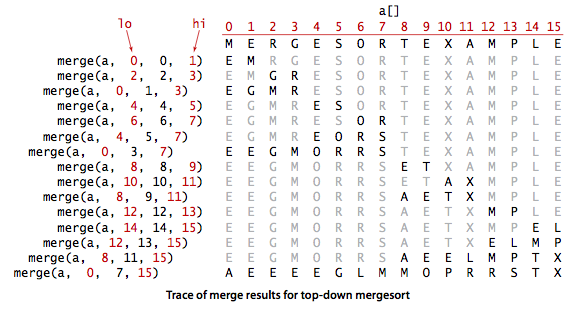
\includegraphics[scale=0.5]{img/mergesortTD.png}
	\caption{Trace of merge results for top-down merge sort.}
\end{figure}

\subsubsection{Bottom-up merge sort}
The list is treated as an array of sublists which are iteratively merged to
form bigger ones.

\lstinputlisting{code/MergeBU.java}

\begin{figure}[ht]
	\centering
	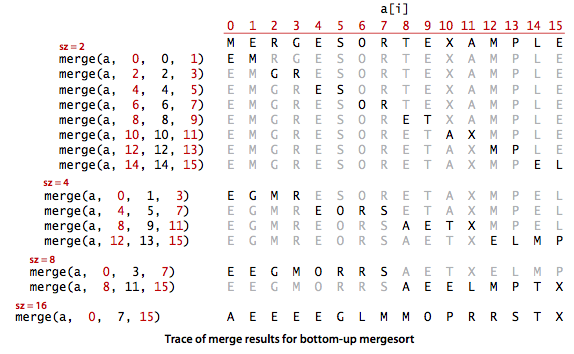
\includegraphics[scale=0.5]{img/mergesortBU.png}
	\caption{Trace of merge results for bottom-up merge sort.}
\end{figure}

This method is preferred for sorting linked lists.

\subsection{Quicksort}
\subsubsection{Principles}
Quicksort is probably the most used sorting algorithm, for the following reasons:
\begin{itemize}
	\item it is an in-place algorithm;
	\item it has a $\bigoh(n \log n)$ complexity.
\end{itemize}

Quicksort is a \textit{divide and conquer} algorithm. It first divides a large
array into two smaller sub-arrays. It can then recursively sort the sub-arrays
as in \figuref{quicksort-overview}.

\begin{figure}[ht]
	\centering
	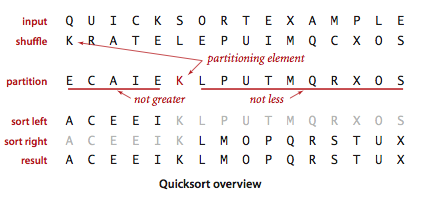
\includegraphics[scale=0.7]{img/quicksort-overview.png}
	\caption{Quicksort overview.}
	\label{fig:quicksort-overview}
\end{figure}

The partitioning algorithm has to rearrange the array such that the following
three conditions are met:

\begin{itemize}
	\item The element \lstinline{a[j]} is in its final position for a certain
	value of $j$. This element is called the pivot;
	\item All elements coming before the pivot (\lstinline{a[lo..j-1]}) have
	values less than or equal to the pivot;
	\item All elements coming after the pivot (\lstinline{a[j+1..hi]}) have
	values greater than or equal to the pivot.
\end{itemize}

These 3 conditions are summarised in \figuref{part-overview}.

\begin{figure}[ht]
	\centering
	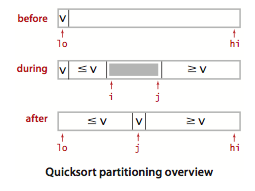
\includegraphics[scale=0.7]{img/partitioning-overview.png}
	\caption{Partitioning overview.}
	\label{fig:part-overview}
\end{figure}

\subsubsection{Implementation}
The trace of the following code is found in \figuref{part-trace}

\lstinputlisting{code/Quick.java}

\begin{figure}[ht]
	\centering
	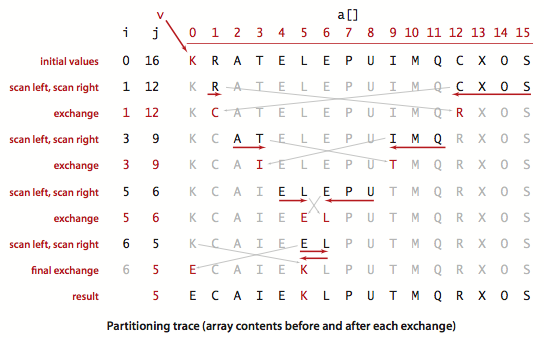
\includegraphics[scale=0.5]{img/partitioning.png}
	\caption{Partitioning trace.}
	\label{fig:part-trace}
\end{figure}

\subsubsection{Complexity}
In the worst case, quicksort has $\bigoh(n^2)$ time complexity. This worst case
scenario can be avoided by randomly ordering the array before sorting it (this
makes quicksort a \emph{randomised} algorithm).

In the average case, quicksort uses $\bigoh(n\log(n))$ time.

\subsection{3-way quicksort}
\subsubsection{Principles}
If the array contains a lot of duplicate elements (for example the \emph{Dutch
National Flag problem}), it is possible to obtain linear time complexity by
modifying the quicksort algorithm slightly.

This can be achieved by using 3 partitions instead of 2, as shown in
\figuref{part3-overview}.

\begin{figure}[ht]
	\centering
	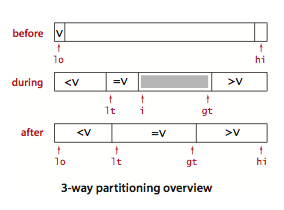
\includegraphics[scale=0.7]{img/partitioning3-overview.png}
	\caption{3-way partitioning overview.}
	\label{fig:part3-overview}
\end{figure}

In order to do this, one must simply scan the array from left to right, while
continuously updating a variable \lstinline{lt} such that
\lstinline{a[lo..lt-1]} are less than $v$, a variable \lstinline{gt} such that
\lstinline{a[gt+1..hi]} are greater than $v$, a variable $i$ such that
\lstinline{a[lt..i-1]} are equal to $v$ and \lstinline{a[i..gt]} have not been
checked yet.

\subsubsection{Implementation}
The trace of the following code is found in \figuref{part3-trace}

\lstinputlisting{code/Quick3way.java}

\begin{figure}[ht]
	\centering
	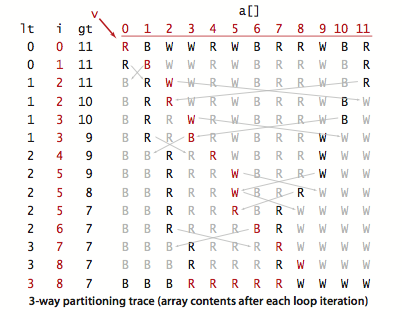
\includegraphics[scale=0.7]{img/partitioning3.png}
	\caption{3-way partitioning trace.}
	\label{fig:part3-trace}
\end{figure}

\begin{table}
\centering
\begin{tabular}{c|c|c|c|c}
	\hline
	\multirow{2}{*}{Algorithm} & \multicolumn{3}{c|}{Time complexity} & Space
	complexity\\
	\cline{2-5}
	 & Best & Average & Worst & Worst\\
	 \hline
	 Quicksort & $\bigomega(n \log n)$ & $\bigtheta(n \log n)$ & $\bigoh(n^2)$
	 & $\bigoh(n \log n)$\\
	 Merge sort & $\bigomega(n \log n)$ & $\bigtheta(n \log n)$ & $\bigoh(n
	 \log n)$ & $\bigoh(n)$\\
	 Insertion sort & $\bigomega(n)$ & $\bigtheta(n^2)$ & $\bigoh(n^2)$ &
	 $\bigoh(1)$\\
	 Selection sort & $\bigomega(n^2)$ & $\bigtheta(n^2)$ & $\bigoh(n^2)$ &
	 $\bigoh(1)$\\
	 Shellsort & $\bigomega(n \log n)$ & $\bigtheta(n (\log n)^2)$ & $\bigoh(n
	 (\log n)^2)$ & $\bigoh(1)$\\
	 \hline
\end{tabular}
\caption{Summary of complexities for sorting algorithms.}
\end{table}

\section{Searching}
\subsection{Symbol tables}
\begin{mydef}[Symbol table]
A \textit{symbol table} is a data structure for key-value pairs that
supports two operations: \textit{insert} (put) a new pair into the
table and \textit{search} for (get) the value associated with a given
key.
\end{mydef}

Here we adopt the \textit{associative array abstraction}, where you can
think of a symbol table as being just like an array where keys are
indices and values are array entries.

The API for a generic basic symbol table is given in \figuref{st-api}.

\begin{figure}[ht]
	\centering
	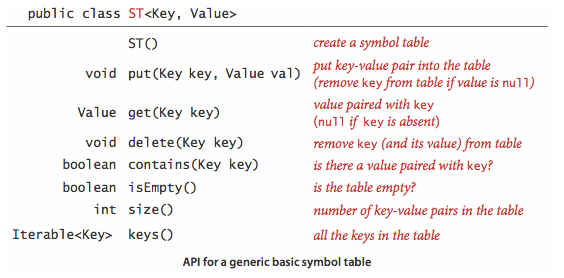
\includegraphics[scale=0.5]{img/symbol-table-api.png}
	\caption{API for a generic basic symbol table.}
	\label{fig:st-api}
\end{figure}

For applications where keys are \lstinline{Comparable}, we usually talk about
\textit{ordered symbol tables}, where keys are kept in order.

The API for a generic ordered symbol table is given in \figuref{ost-api}.

\begin{figure}[ht]
	\centering
	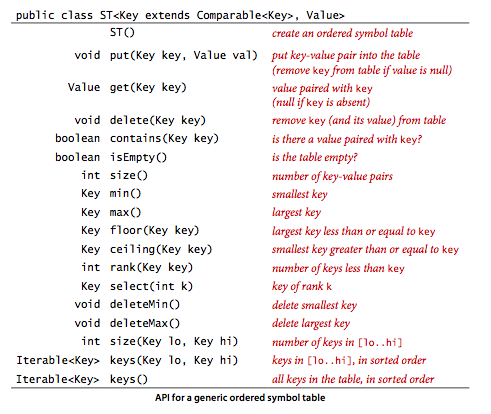
\includegraphics[scale=0.5]{img/ordered-symbol-table-api.png}
	\caption{API for a generic ordered symbol table.}
	\label{fig:ost-api}
\end{figure}

\subsubsection{Sequential search in an unordered linked list}
One straightforward option for the underlying data structure for a
symbol table is a linked list of nodes that contain keys and values.

Implementations of both \lstinline{get()} and \lstinline{put()} consist
of scanning through the list. Hence, it is easy to show that the worst
case complexity is $\bigoh(n)$ for both. In conclusion, a linked list
implementation with sequential search is too slow to be used to solve
huge problems.

\subsubsection{Binary search in an ordered array}

\lstinputlisting{code/BinarySearchSTClass.java}

Now, we consider a full implementation of our ordered symbol-table API.
The underlying data structure is a pair of parallel arrays, one for the
keys and one for the values.

\lstinputlisting{code/BinarySearchST.java}

The heart of the implementation is the \lstinline{rank()} method, which
returns the number of keys smaller than a given key. For \lstinline{get()},
the rank tells us precisely where the key is to be found if it is in the table.

\lstinputlisting{code/Get.java}

For \lstinline{put()}, the rank tells us precisely where to update the value
when the key is in the table, and precisely where to put the key when the
key is not in the table. We move all larger keys one position to the right to
make room and insert the given key and value into the proper positions in their
respective arrays.

\lstinputlisting{code/Put.java}

To find the rank of a given key, we take advantage of the fact that keys
in the array are ordered and use \textit{binary search}. An iterative
implementation of the \lstinline{rank()} method is given below.

\lstinputlisting{code/Rank.java}

Here, it is easy to show that the complexity of binary search
is $\bigoh(n \log n)$. Unfortunately, insertion is still
too slow: $\bigoh(n)$.

\subsection{Binary search tree}
\label{sec:tree}
Here we'll combine the flexibility of insertion in a linked list
with the efficiency of \emph{search} in an ordered array.

\begin{mydef}[Binary Search Tree (BST)]
A \textit{binary search tree} (BST) is a binary tree where each node
has a \lstinline{Comparable} key (and an associated value) and
satisfies the restriction that the key in any node is larger than
the keys in all nodes in that node's left subtree and smaller
than the keys in all nodes in that node's right subtree.
\end{mydef}

This restriction is illustrated in \figuref{bst-anatomy}.
Note that on a binary tree that is not a binary \textit{search}
tree, we don't have this restriction.

\begin{figure}[ht]
	\centering
	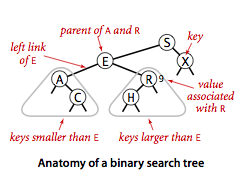
\includegraphics[scale=0.65]{img/bst-anatomy.png}
	\caption{BST anatomy.}
	\label{fig:bst-anatomy}
\end{figure}

\begin{myrem}
It's interesting to note that there are many different BSTs that
represent the same set.
\end{myrem}

\subsubsection{Basic implementation}
\lstinputlisting{code/BSTClass.java}

Just as we did for linked lists, we define a private nested class
to define nodes in BSTs.

\lstinputlisting{code/NodeClass.java}

Each node contains a key, a value, a left and right link and a node
count. This last field facilitates the implementation of various
ordered symbol table operations.

\lstinputlisting{code/Size.java}

Thanks to the recursive definition of a tree, we can implement
the \lstinline{get()} method easily in a recursive way.

\lstinputlisting{code/NodeGet.java}

The same holds for the \lstinline{put()} method.

\lstinputlisting{code/NodePut.java}

To get a better understanding of the dynamics of these
recursive implementations, you can think of the code
\textit{before} the recursive calls as happening on the
way \textit{down} the tree. Then, think of the code \textit{after}
the recursive calls as happening on the way \textit{up} the tree.

Now, let's look at how to delete a node in a BST. This is the most
difficult operation to implement. We choose here to use the
\textit{Hibbard deletion}. With this method, we delete a node
$x$ by replacing it with its \textit{successor}. If $x$ has
a right child, its successor is the node with the smallest
key in its right subtree. This task is accomplished
in 4 steps:

\begin{itemize}
	\item save a link to the node to be deleted in \lstinline{t};
	\item set \lstinline{x} to point to its successor
	\lstinline{min(t.right)};
	\item set the right link of \lstinline{x} to
	\lstinline{deleteMin(t.right)};
	\item set the left link of \lstinline{x} to \lstinline{t.left}.
\end{itemize}

\lstinputlisting{code/HibbardDeletion.java}

Even though this method does the job, it has a flaw that might
cause performance issues in some practical situations. The problem
is that the choice of using the successor is arbitrary and not
symmetric. This will cause the BST to become skewed toward the
left on the long term for random deletions and insertions
\footnote{See the last video on
\url{http://algs4.cs.princeton.edu/32bst/}.}.

\begin{myrem}
Note that deletion in a BST is not commutative. Try for
example to delete 4 and then 3 and 3 and then 4 in
the tree given in \figuref{nc-deletion}.

\begin{figure}[ht]
	\centering
	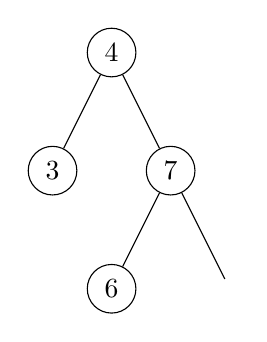
\begin{tikzpicture}
		\node [circle,draw] {4}
		child {node [circle,draw] {3}}
		child {node [circle, draw] {7}
			child {node [circle,draw] {6}}
			child {node [] {}}};
	\end{tikzpicture}
	\caption{Example of non-commutative deletion.}
	\label{fig:nc-deletion}
\end{figure}
\end{myrem}

\begin{myrem}
Other methods from the API are in the book.
\end{myrem}

\subsubsection{Analysis}
The running times of algorithms on binary search trees depend
on the shapes of the trees, which in turn, depend on the
order in which keys are inserted. In the best case, a tree
with $N$ nodes could be perfectly balanced, with $\lg N$
nodes between the root and each null link (we call this the
\textit{depth} of a tree). In the worst case
there could be $N$ nodes on the search patch.

\begin{mypropo}
Search hits in a BST built from $N$ random keys requires $\sim 2\ln N$
(about $1.39 \lg N$) compares on the average.
\end{mypropo}

\begin{mypropo}
Insertion and search misses in a BST built from $N$ random
keys require $\sim 2\ln N$ (about $1.39 \lg N$) compares on the
average.
\end{mypropo}

\begin{mypropo}
Search, insertion, finding the maximum, floor, ceiling, rank, select, delete
the minimum, delete the maximum, delete, and range count operations all take
time proportional to the height of the tree, in the worst case.
\end{mypropo}

\subsubsection{Binary tree traversal methods}
We will use the BST given in \figuref{bst-anatomy}
for the following examples and assume that the method
\lstinline$void visit(Node h)$ prints the key of node
\lstinline$h$.

\paragraph{Preorder (\textit{préfixe)}}
Visit a node, then its left child and right child.
\lstinputlisting{code/Preorder.java}
Applied on \figuref{bst-anatomy} :
S E A C R H X.

\paragraph{Inorder (\textit{infixe})}
This method is equivalent to projecting the keys
of the tree on a line at the bottom of the tree :
\textbf{keys appear in sorted order}.

\lstinputlisting{code/Inorder.java}
Applied on \figuref{bst-anatomy} :
A C E H R S X.

\paragraph{Postorder (\textit{postfixe} ou \textit{suffixe})}
Visit each node after having visited each child.
\lstinputlisting{code/Postorder.java}
Applied on \figuref{bst-anatomy} :
C A R H E X S.

\subsection{Balanced search tree}
The algorithms in the previous subsection have poor worst case
performance. Here we introduce a type of binary search tree where
costs are \textit{guaranteed} to be logarithmic. Ideally, we would
like to keep our binary search tree perfectly balanced, i.e. in an
$N$-node tree, we would like the height to be $\lg N$. Unfortunately,
maintaining this property is too expensive. Hence we will consider
a data structure that slightly relaxes the perfect balance
requirement to provide guaranteed logarithmic performance.

\begin{mydef}[2-3 search tree]
A \textit{2-3 search tree} is a tree that is either empty or
\begin{itemize}
	\item a \textit{2-node}, with one key (and associated value)
	and two links, a left link to a 2-3 search tree with smaller
	keys, and a right link to a 2-3 search tree with larger keys;
	\item a \textit{3-node}, with two keys (and associated values)
	and \textit{three} links, a left link to a 2-3 search tree with
	smaller keys, a middle link to a 2-3 search tree with keys
	between the node's keys, and a right link to a 2-3 search tree
	with larger keys.
\end{itemize}
As usual, we refer to a link to an empty tree as a \textit{null link}.
\end{mydef}

\begin{myprop}[Perfectly balanced 2-3 search tree]
A \textit{perfectly balanced} 2-3 search tree is one whose null
links are all the same distance from the root.
\end{myprop}

Searching in a 2-3 search tree is almost the same as searching
in a BST. The only difference occurs when we encounter a 3-node,
instead of just looking if the target key is smaller or larger
than the keys, we also have to check if the target key is
between the two keys of the 3-node.

Inserting in a 2-3 search tree is more complicated. The primary reason
that 2-3 trees are useful is that we can do insertions and still
maintain perfect balance. To achieve this, we have to take into
account different cases illustrated below
(see \figuref{23tree-inserta}, \figuref{23tree-insertb}
and \figuref{23tree-insertc}).

\begin{mypropo}
Transformations caused by the 2-3 tree insertion algorithms
are purely \textit{local}: no part of the tree needs to be examined
or modified other than the specified nodes and links. Moreover, these
local transformations preserve the global properties that the tree
is ordered and perfectly balanced.
\end{mypropo}

\begin{mypropo}
Search and insert operations in a 2-3 tree with $N$ keys are
guaranteed to visit at most $\lg N$ nodes. Indeed, the height
of an $N$-node 2-3 tree is between $\log_3 N$ (if the tree is
all 3-nodes) and $\lg N$ (if the tree is all 2-nodes).
\end{mypropo}

\begin{figure}[ht]
	\centering
	\begin{subfigure}[t]{.5\textwidth}
		\centering
  		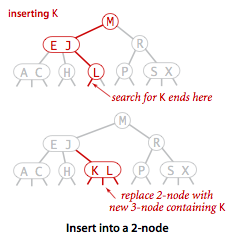
\includegraphics[width=.7\linewidth]{img/23tree-insert2.png}
 		\caption{Inserting into a 2-node.}
  		\label{fig:23tree-insert2}
	\end{subfigure}%
	\begin{subfigure}[t]{.5\textwidth}
  		\centering
  		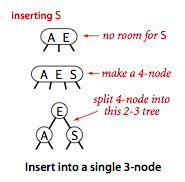
\includegraphics[width=0.5\linewidth]{img/23tree-insert3a.png}
  		\caption{Inserting into a single 3-node.}
  		\label{fig:23tree-insert3a}
	\end{subfigure}
	\caption{}
	\label{fig:23tree-inserta}
\end{figure}

\begin{figure}[ht]
	\centering
	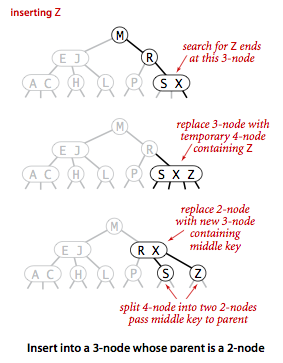
\includegraphics[scale=0.55]{img/23tree-insert3b.png}
	\caption{}
	\label{fig:23tree-insertb}
\end{figure}

\begin{figure}[ht]
	\centering
	\begin{subfigure}[t]{.5\textwidth}
		\centering
  		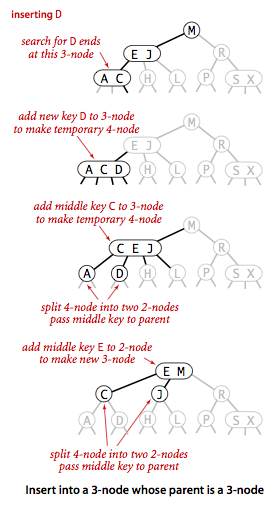
\includegraphics[width=.7\linewidth]{img/23tree-insert3c.png}
 		\caption{Insert intro a 3-node whose parent is a 3-node.}
  		\label{fig:23tree-insert3c}
	\end{subfigure}%
	\begin{subfigure}[t]{.5\textwidth}
  		\centering
  		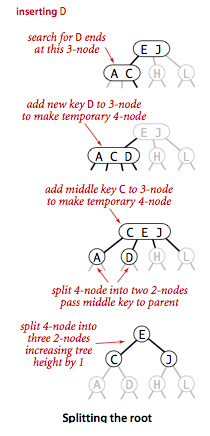
\includegraphics[width=0.6\linewidth]{img/23tree-split.png}
  		\caption{Splitting the root.}
  		\label{fig:23tree-split}
	\end{subfigure}
	\caption{}
	\label{fig:23tree-insertc}
\end{figure}

\subsubsection{Implementation}
To implement a 2-3 tree, we consider a simple representation
known as \textit{red-black BST}. The basic idea behind red-black
BSTs is to encode 2-3 trees by starting with standard BSTs and adding
extra information to encode 3-nodes. We think of the links as being of
two different types: \textit{red} links, which bind together two 2-nodes
to represent a 3-node, and \textit{black} links, which bind together
the 2-3 tree. Specifically, we represent 3-nodes as two 2-nodes connected
by a single red link that leans left. This is illustrated in
\figuref{redblack-encoding}.

One advantage of using such a representation is that it allows us
to use our \lstinline$get()$ code for standard BST search without
modification.

\begin{mydef}[Equivalent definition]
A red-black BST is a BST having red and black links and satisfying
the following three restrictions:
\begin{itemize}
	\item red links lean left;
	\item no node has two red links connected to it;
	\item the tree has \textit{perfect black balance}: every path from
	the root to a null link has the same number of black links - we refer
	to this number as the tree's \textit{black height}.
\end{itemize}
\end{mydef}

\begin{mypropo}
\label{correspondence}
There is a 1-1 correspondence between red-black BSTs and 2-3 trees.
\end{mypropo}

Proposition \ref{correspondence} is illustrated in \figuref{redblack-1-1}.

\begin{figure}[ht]
	\centering
	\begin{subfigure}[t]{.48\textwidth}
		\centering
		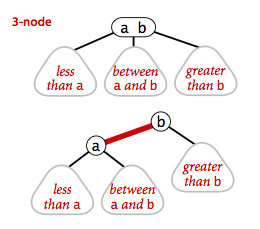
\includegraphics[scale=0.5]{img/redblack-encoding.png}
		\caption{Encoding a 3-node with two 2-nodes connected by
		a left leaning red link.}
		\label{fig:redblack-encoding}
	\end{subfigure}%
	\hfill
	\begin{subfigure}[t]{.48\textwidth}
		\centering
		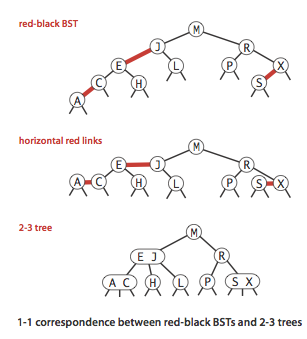
\includegraphics[scale=0.5]{img/redblack-1-1.png}
		\caption{1-1 correspondence between red-black BSTs and 2-3 trees.}
		\label{fig:redblack-1-1}
	\end{subfigure}
	\caption{}
	\label{fig:redblack-principles}
\end{figure}

\lstinputlisting{code/RedBlackBST.java}

As usual, we define a private nested class to define a node.

\lstinputlisting{code/RedBlackNode.java}

When we refer to the color of a node, we are referring
to the color of the link pointing to it. By convention, null
links are black. Now we consider two methods
\lstinline$Node rotateLeft(Node h)$ and \lstinline$Node rotateRight(Node h)$.
These two methods will help us to write other methods later. They
are illustrated in \figuref{redblack-left-rotate} and
\figuref{redblack-right-rotate}.

\begin{figure}[ht]
	\centering
	\begin{subfigure}[t]{.5\textwidth}
		\centering
		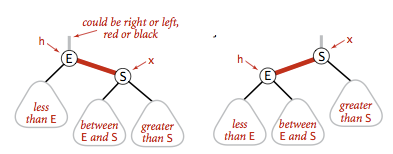
\includegraphics[scale=0.5]{img/redblack-left-rotate.png}
		\caption{Left rotate.}
		\label{fig:redblack-left-rotate}
	\end{subfigure}%
	\begin{subfigure}[t]{.5\textwidth}
		\centering
		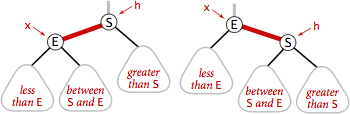
\includegraphics[scale=0.5]{img/redblack-right-rotate.png}
		\caption{Right rotate.}
		\label{fig:redblack-right-rotate}
	\end{subfigure}
	\caption{}
	\label{fig:redblack-rotations}
\end{figure}

\lstinputlisting{code/NodeRotate.java}

Next we consider a simple method which allows us to
split a 4-node.

\lstinputlisting{code/FlipColors.java}

This method is illustrated in \figuref{color-flip}.

\begin{figure}[ht]
	\centering
	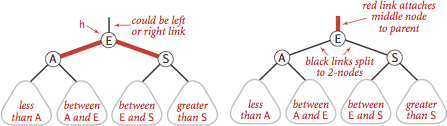
\includegraphics[scale=0.55]{img/color-flip.png}
	\caption{Flipping colors to split a 4-node.}
	\label{fig:color-flip}
\end{figure}

With the last three methods, we have everything we need to
implement insertion in red-black BSTs.

\lstinputlisting{code/RedBlackPut.java}

A summary of rotations and colors flipping involved in insert is
given in figure \ref{fig:insert-summary}.

\begin{figure}[ht]
	\centering
	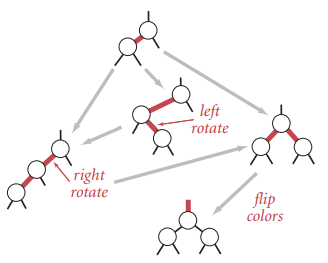
\includegraphics[scale=0.55]{img/insert-summary.png}
	\caption{Operations involved in insert.}
	\label{fig:insert-summary}
\end{figure}

% TODO : deletion in a red-black BST

\subsubsection{Analysis}
\begin{mypropo}
The height\footnote{Here we are not talking about black height!}
of a red-black BST with $N$ nodes
is no more than $2\lg N$. Indeed, the worst case
is a 2-3 tree that is all 2-nodes except that the leftmost
is made up of 3-nodes. The path taking left links from the
root is twice as long as the path of length $\sim \lg N$
that involves just 2-nodes.
\end{mypropo}

The worst case of the last proposition corresponds to the first
tree of \figuref{redblack-1-1} with $S$ removed.

\begin{myprop}
The average length of a path from the root to a node
in a red-black BST with $N$ nodes is $\sim 1.00\lg N$.
\end{myprop}

\begin{mypropo}
In a red-black BST, the following operations take logarithmic time
in the worst case: search, insertion, finding the minimum/maximum,
floor, ceiling, rank, select, delete the minimum/maximum, delete
and range count.
\end{mypropo}

\subsection{Hash tables}

If keys are small integers, we can use an array to implement
an unordered symbol table, by interpreting the key as an array
index so that we can store the value associated with the key
\lstinline$i$ in array position \lstinline$i$, ready for
\textbf{immediate access}. Thanks to \emph{hashing}, we can
transform any type of key to array indexes. Ideally, different
keys would map to different indices. However, this ideal
is generally beyond our reach, so we have to face the possibility
that two or more different keys may hash to the same array index:
we need a \textit{collision resolution} process. We'll consider
two different approaches to collision resolution: \textit{separate
chaining} and \textit{linear probing}.

\subsubsection{Hash functions}

\begin{wrapfigure}{r}{0.3\textwidth}
  \begin{center}
    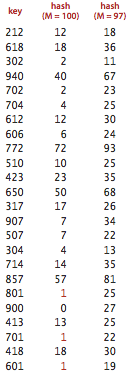
\includegraphics[width=0.15\textwidth]{img/modular-hashing.png}
  \end{center}
  \caption{Modular hashing.}
  \label{fig:modular-hashing}
\end{wrapfigure}

If we have an array that can hold $M$ key-value pairs, then we
need a hash function that can transform any given key into an
integer in the range $\intervalcc{0}{M-1}$. We seek a hash function that is both
\textbf{efficient to compute} and \textbf{uniformly distributes}
the keys.

\paragraph{Hashing positive integers}
The most commonly used method for hashing integers is called
\textit{modular hashing}: we choose the array size $M$ to be prime
and, for any positive integer key $k$, compute the remainder
when dividing $k$ by $M$ : $k \bmod M$.

If $M$ is not prime, it may be the case that not all the bits
of the key play a role, which amounts to missing an opportunity
to disperse the values evenly. For example, if the keys are
base 10 numbers and $M$ is $10^k$, then only the $k$ least
significant digits are used (see \figuref{modular-hashing}).

\paragraph{Hashing floating-point numbers}
One way to do this is to use modular hashing on the binary
representation of the key (this is what \java{} does).

\paragraph{Hashing strings}
Again, we can apply modular hashing on each character of
the string :

\lstinputlisting{code/Horner.java}

This algorithm is called \textit{Horner's method}.
The use of a small prime integer such as 31 ensures
that the bits of all the characters play a role.

\begin{myrem}
\label{rem:mod-prop}
Note that applying $\mod M$ at the end (i.e. outside
the loop) gives the same result (it's a property of the
modulus operation). But by doing so, we may encounter
\lstinline|int| overflow for long strings.
\end{myrem}

\paragraph{\java{} conventions}
In \java, every data type inherits a method called
\lstinline$hashCode()$ that returns a 32-bit integer.
The implementation of \lstinline$hashCode()$ for a data
type must be \textbf{consistent with equals}, if
\lstinline$a.equals(b)$, then \lstinline$a.hashCode()$
must have the same numerical value as
\lstinline$b.hashCode()$. Conversely, if
\lstinline$hashCode()$ values
are different, then objects are different. \textbf{But},
if \lstinline$hashCode()$ values are the same, we still
have to use \lstinline$equals()$ to check whether or not
objects are equal (as collisions may occur).

\paragraph{Converting a \lstinline$hashCode()$ to an array index}
Since our goal is an array index, not a 32-bit integer, we
combine \lstinline$hashCode()$ with modular hashing
to produce integers between 0 and $M-1$ :

\lstinputlisting{code/Hash.java}

This code also masks off the sign bit (to turn the
32-bit number into a 31-bit non-negative integer).
We usually use a prime number for the hash table
size $M$ to attempt to make use of all the bits of
the \lstinline$hashCode()$.

\paragraph{Software caching}
If computing the \lstinline$hashCode()$ is expensive, it may be
worthwhile to \textit{cache the hash} for each key.
That is, we maintain an instance variable \lstinline$hash$
in the key type that contains the value of
\lstinline$hashCode()$ for each key object. \java{} uses
this technique for \lstinline$String$ objects.

\subsubsection{Hashing with separate chaining}
Now that we know how to hash, we need a collision resolution
process. The first collision resolution process is illustrated
in \figuref{separate-chaining}.

\begin{figure}[ht]
	\centering
	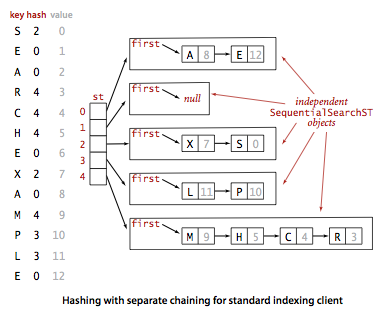
\includegraphics[scale=0.6]{img/separate-chaining.png}
	\caption{For each of the $M$ array indices, we build a
	linked list of the key-value pairs  whose key hashes to that
	index. To search in those linked lists, we use sequential
	search in an unordered linked list.}
	\label{fig:separate-chaining}
\end{figure}

\paragraph{Implementation}
Implementation of separate chaining is very easy
(\lstinline|SequentialSearchST| is the implementation
of the sequential search in an unordered linked list).

\lstinputlisting{code/SeparateChaining.java}

\paragraph{Analysis}
\begin{mypropo}
In a separate-chaining hash table with $M$ lists and $N$
keys, the probability that the number of keys in a list
is within a small constant factor of $N/M$ is extremely
close to 1.
\end{mypropo}

This last proposition makes the assumption that we use
a uniform hashing function.

\begin{myprop}
As a consequence of the last proposition, the number of
compares for \emph{search} and \emph{insert} is proportional to $N/M$.
\end{myprop}

\subsubsection{Hashing with linear probing}
Another approach to implementing hashing is to store
$N$ key-value pairs in a hash table of size $M > N$,
relying on empty entries in the table to help with
collision resolution. Such methods are called
\textit{open-addressing} hashing methods. The simplest
one is called linear probing: when there is a collision,
then we just check the next entry in the table.

\paragraph{Implementation}
As with separate chaining, implementation is quite
straightforward.

\lstinputlisting{code/LinearProbing.java}

\begin{mydef}[Load factor]
We define $\alpha = N/M$ as the \textit{load factor}
of a hash table. For separate chaining, $\alpha$ is
the average number of keys per list and is often
larger than 1. For open addressing, $\alpha$ is the
percentage of table entries that are occupied: it
\emph{must} be less than 1.\footnote{If the load
factor reaches 1, search misses would go into an
infinite loop.}
\end{mydef}

The average cost of linear probing depends on \textit{clusters}
(entries which clump together into contiguous groups).
For the sake of good performance, we use array resizing
to guarantee that the load factor is between $\frac{1}{8}$
and $\frac{1}{2}$: this allows us to avoid too long clusters.
The \lstinline|resize| method is given below.

\lstinputlisting{code/Resize.java}


\subsection{Summary}
The cost-summary for symbol-tables implementations is given
in \tabref{cost-summary-searching}.

% auto-generated from here http://www.tablesgenerator.com/ #flemme
\begin{table}[ht]
\centering
\begin{tabular}{c|cccc|c}
\multirow{2}{*}{\begin{tabular}[c]{@{}c@{}}algorithm \\(data
structure)\end{tabular}} &
\multicolumn{2}{c}{\begin{tabular}[c]{@{}c@{}}worst-case cost\\ (after N
inserts)\end{tabular}} &
\multicolumn{2}{c|}{\begin{tabular}[c]{@{}c@{}}average-case cost\\ (after N
random inserts)\end{tabular}} &
\multirow{2}{*}{\begin{tabular}[c]{@{}c@{}}efficiently supports\\ordered
operations?\end{tabular}} \\
\cline{2-5}
& search & insert & search hit & insert &  \\ \hline
\begin{tabular}[c]{@{}c@{}}sequential search\\
(unordered linked list)\end{tabular} & $N$ & $N$ & $N/2$ & $N$ & no  \\
\cline{1-1}
\begin{tabular}[c]{@{}c@{}}binary search\\
(ordered array)\end{tabular} & $\lg N$ & $N$ & $\lg N$ & $N/2$ & yes \\
\cline{1-1}
\begin{tabular}[c]{@{}c@{}}binary tree search\\
(BST)\end{tabular} & $N$ & $N$ & $1.39 \ln N$ & $1.39 \ln N$ & yes \\
\cline{1-1}
\begin{tabular}[c]{@{}c@{}}2-3 tree search\\
(red-black BST)\end{tabular} & $2 \lg N$ & $2 \lg N$ & $1.00 \lg N$ & $1.00 \lg
N$ & yes \\
\cline{1-1}
\begin{tabular}[c]{@{}c@{}}separate chaining\\
(array of lists)\end{tabular} & $N$ & $N$ & $\frac{N}{2M}$ & $N/M$ & no \\
\cline{1-1}
\begin{tabular}[c]{@{}c@{}}linear probing\\
(parallel arrays)\end{tabular} & $N$ & $N$ & $< 1.50$ & $< 2.50$ & no
\end{tabular}
\caption{Cost summary for symbol-table implementations.}
\label{tab:cost-summary-searching}
\end{table}

\section{Strings}
\subsection{Tries}
\paragraph{Goals}
As with sorting, we can take advantage of properties of strings to develop
search methods (symbol-table implementations) that can be more efficient for
typical applications where search keys are strings. More specifically, the
goals are the following ones:

\begin{itemize}
\item{search hits take time proportional to the length of the search key;}
\item{search misses involve examining only a few characters.}
\end{itemize}

To achieve them, we have to adjust the symbol-table API (\figuref{triesAPI}) to
provide specific character-based operations for string keys.

\begin{figure}[ht!]
\centering
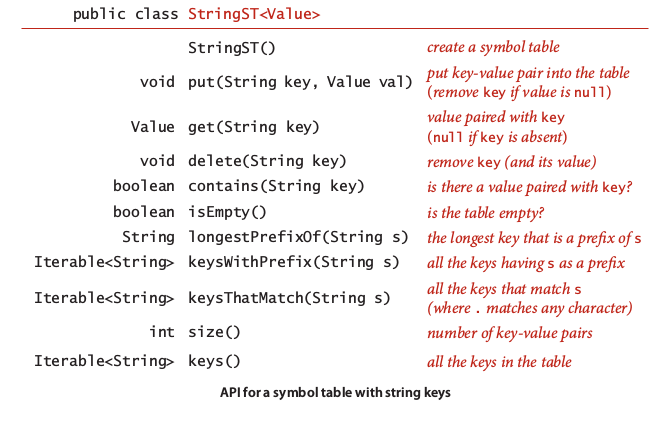
\includegraphics[width=.7\linewidth]{img/APItries.png}
\caption{Tries API.}
\label{fig:triesAPI}
\end{figure}

Considering the following example keys:
\lstinline|she sells sea shells by the sea shore|. Let's focus on the addition
of three new methods.

\begin{itemize}
\item{\lstinline$longuestPrefixOf()$ takes a string as argument and returns the
longest key in the symbol table that is a prefix of that string. For the given
keys, \lstinline$longestPrefixOf("shell")$ is \lstinline$she$ and
\lstinline$longestPrefixOf("shellsort")$ is \lstinline$shells$.}
\item{\lstinline$keysWithPrefix()$ takes a string as argument and returns all
the keys in the symbol table having that string as prefix. For the given keys,
\lstinline$keysWithPrefix("she")$ is \lstinline$she$ and \lstinline$shells$,
and \lstinline$keysWithPrefix("se")$ is \lstinline$sells$ and \lstinline$sea$.}
\item{\lstinline$keysThatMatch()$ takes a string as argument and returns all
the keys in the symbol table that match that string, in the sense that a period
(\lstinline$.$) in the argument string matches any character. For the given
keys, \lstinline$keysThatMatch(".he")$ returns \lstinline$she$ and
\lstinline$the$, and \lstinline$keysThatMatch("s..")$ returns \lstinline$she$
and \lstinline$sea$.}
\end{itemize}

\subsubsection{Basic tries}

\begin{mydef}[Trie]
A \textit{trie} is a search tree built from the characters of the string keys
that allows us to use the characters of the search key to guide the search. A
trie has the same structure as a search tree. We usually omit null links due to
a substantial number of these ones. Each node corresponds to a character value
(except the root) and is associated to a value, which can be \textit{null} or
the value associated to one of the string keys of the symbol table. A
representation is given in \figuref{basic_trie}.
\end{mydef}


\begin{figure}[ht!]
\centering
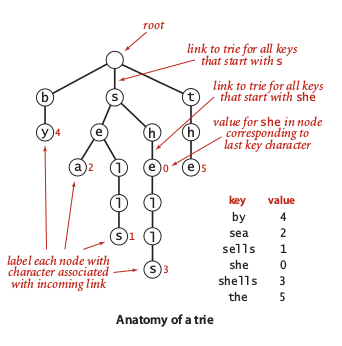
\includegraphics[width=.4\linewidth]{img/tries.png}
\caption{Basic trie.}
\label{fig:basic_trie}
\end{figure}

\paragraph{Search}
Due to this organisation, \emph{search} in tries is very easy: beginning at the
root, following the path made by the characters inside the nodes until reaching
the last character of the key is the only thing you have to do. Null links may
be found if the next desired character isn't in the trie. Three results can
occur:

\begin{itemize}
\item{The value at the node corresponding to the last character in the key is
not \lstinline$null$: this result is a \textbf{search hit}. The value
associated with the key is the value in the node corresponding to its last
character.}
\item{The value in the node corresponding to the last character in the key is
\lstinline$null$ (as in the search for \lstinline$shell$ depicted in the top
right of \figuref{basic_trie}). This result is a \textbf{search miss}: the key
is not in the table.}
\item{The search terminated with a null link (as in the search for
\lstinline$shore$ depicted in the bottom right of \figuref{basic_trie}). This
result is also a \textbf{search miss}.}
\end{itemize}

\paragraph{Node representation}
\begin{itemize}
	\item{Every node has R links, one for each possible character.}
	\item{Characters and keys are implicitely stored in the data structure.}
\end{itemize}

An example of search is given in \figuref{basic_trie_search}.

\begin{figure}[ht!]
\centering
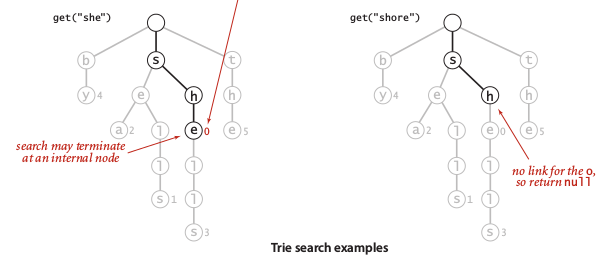
\includegraphics[width=.75\linewidth]{img/trieSe.png}
\caption{Search in a basic trie.}
\label{fig:basic_trie_search}
\end{figure}

\paragraph{Insertion}
To insert a value, we begin by doing a search: we go down the trie, guided by
the character of the key. Two situations can occur:

\begin{itemize}
\item{\textbf{Null link encountered}: a null link is encountered before
reaching the last character of the key. This implies that there is no node
corresponding to this one and we thus have to create a new node for each
remaining character of the key. The value is set in the node of the last
character.}
\item{\textbf{Last character encountered}: the last character of the key is
encountered before reaching a null link. We just have to set the node's value
to the value corresponding to the key.}
\end{itemize}

An example of insertion in a basic trie is given in
\figuref{basic_trie_insertion}.

\begin{figure}[ht!]
\centering
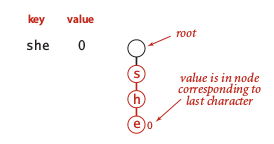
\includegraphics[width=.4\linewidth]{img/trieIn1.png}\hfill
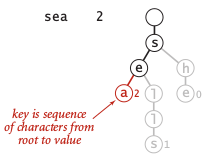
\includegraphics[width=.3\linewidth]{img/trieIn2.png}\hfill
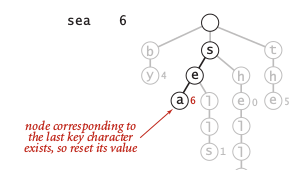
\includegraphics[width=.4\linewidth]{img/trieIn3.png}
\caption{Insertion in a basic trie.}
\label{fig:basic_trie_insertion}
\end{figure}

\paragraph{Implementation}
An implementation of a trie is given below:
\lstinputlisting{code/TrieST.java}

\paragraph{Collecting keys}
Because keys are represented implicitly in the trie, it is difficult to provide
the user with the ability to iterate through the keys. We do not use a queue to
store the different keys as with the binary search tree but we create an
explicit representation of all the string keys using the recursive method
\lstinline$collect()$. This method visits the different nodes and appends the
corresponding characters to create the keys. The \lstinline$collect()$ method
is used to implement the \lstinline$keysWithPrefix()$ method which is used to
implement the \lstinline$keys()$ method. The last one allows to create all the
different keys (example given in \figuref{keysRe}). An implementation of the
\lstinline$collect()$, \lstinline$keysWithPrefix()$ and \lstinline$keys()$
methods is given below:

\lstinputlisting{code/KeysWithPrefix.java}

The \lstinline$keysThatMatch()$ method uses a similar process, but adds an
argument to specify the pattern to collect. A possible implementation is given
below:

\lstinputlisting{code/KeysThatMatch.java}

The \lstinline$longestPrefixOf()$ method first looks for the biggest length
found for a path that matches with the parameter string and then returns a
substring with the obtained length. See code below:

\lstinputlisting{code/LongestPrefixOf.java}

\begin{figure}[ht!]
\centering
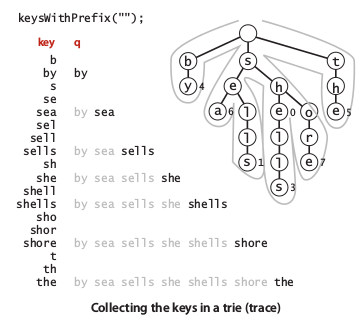
\includegraphics[width=.45\linewidth]{img/keysRe.png}
\caption{Key recuperation.}
\label{fig:keysRe}
\end{figure}

\paragraph{Deletion}
As for insertion, the first step of deletion is a search: the goal is to find
the node corresponding to the key and set its value to null. Two situations may
occur then:

\begin{itemize}
\item{the node has a non-null link to a child. No more work is required;}
\item{all the remaining links are null. We thus have to remove the node.
Caution needs to be taken that if doing so leaves all the links null in its
parent, we need to remove that node, and so forth.}
\end{itemize}
An example is given in \figuref{trieDel}. A possible implementation is
given below:
\lstinputlisting{code/TrieDelete.java}

\begin{figure}[ht!]
\centering
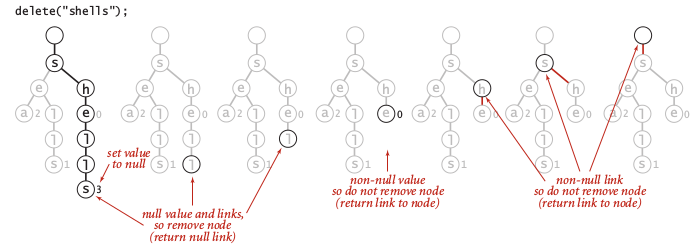
\includegraphics[width=.75\linewidth]{img/trieDel.png}
\caption{Deletion with basic trie.}
\label{fig:trieDel}
\end{figure}

\begin{mypropo}
The linked structure (shape) of a trie is independent of the key
insertion/deletion order: there is a unique trie for any given set of keys.
\end{mypropo}

\begin{mypropo}
The number of array accesses when searching in a trie or inserting
a key into a trie is at most 1 plus the length of the key. From a theorical
point of view, this implies that tries are optimal for search hits.
\end{mypropo}

\begin{mypropo}
The average number of nodes examined for a search miss in a trie
built from $N$ random keys over an alphabet of size $R$ is $\sim \log R N$.
\end{mypropo}

\begin{mypropo}
The number of links in a trie is between $RN$ and $RNw$, where $w$ is
the average key length. More precisely, for $N$ random keys and $w$ the average
length of a key, we can prove that:
\begin{itemize}
\item{when keys are short, the number of links is close to $RN$;}
\item{when keys are long, the number of links is close to $RNw$;}
\item{therefore, decreasing $R$ can save a huge amount of space.}
\end{itemize}
\end{mypropo}

\paragraph{Size}
On average, the required space for a trie is huge due to the one-way-branching
that can occur. A solution to this problem is the \textit{ternary search trie}.

\subsubsection{Ternary search tries (TST)}

\begin{mydef}[Ternary Search Trie (TST)]
A \textit{ternary search trie} is a trie in which each node has a character,
three links, and a value. The three links correspond to keys whose current
characters are less than, equal to, or greater than the node’s character. In a
TST, characters appear explicitly in nodes: we find characters corresponding to
keys only when we are traversing the middle links.
\end{mydef}

\paragraph{Search}
Due to this configuration, \emph{search} appears to be easy: we compare the
first character in the key with the character at
the root. If it is less, we take the left link; if it is
greater, we take the right link; and if it is equal,
we take the middle link and move to the next
search key character. The algorithm is applied recursively.

\paragraph{Insertion}
The insertion is like an insertion for tries: beginning with a search and then
add the value in a new node or not. A example is given in \figuref{TSTSe}.

\begin{figure}[ht!]
\centering
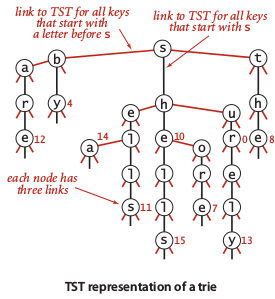
\includegraphics[width=.4\linewidth]{img/TST.png}
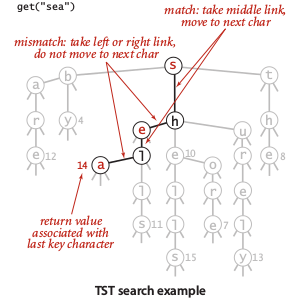
\includegraphics[width=.4\linewidth]{img/TSTSe.png}
\caption{TST representation and search.}
\label{fig:TSTSe}
\end{figure}

Using this arrangement is equivalent to implementing
each R-way trie node as a binary search tree that uses
as keys the characters corresponding to non-null links.
Continuing the correspondence, TSTs correspond to 3-way string quicksort
(\figuref{TSTnode}).

\begin{figure}[ht!]
\centering
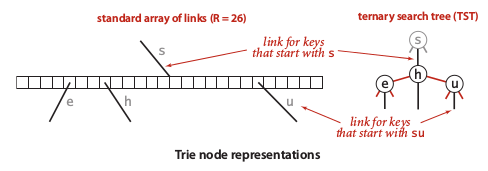
\includegraphics[width=.75\linewidth]{img/TSTnode.png}
\caption{Node representation of a TST.}
\label{fig:TSTnode}
\end{figure}

\paragraph{Implementation}
An implementation is given below:

\lstinputlisting{code/TST.java}

\begin{mypropo}
The number of links in a TST built from $N$ string keys of average
length $w$ is between $3N$ and $3Nw$. This implies that the required space for
a TST is well-over shorter than for a basic trie.
\end{mypropo}

\begin{mypropo}
A search miss in a TST built from $N$ random string keys requires on the
average $\sim \ln N$ character compares: a search hit or an insertion in a TST
uses a character compare for each character in the search key.
\end{mypropo}

In the worst case, a node might be a full R-way node that is unbalanced,
stretched out like a singly linked list, so we would need to multiply by a
factor of $R$.

\paragraph{Alphabets}
The prime virtue of using TSTs is that they adapt gracefully to irregularities
in search keys. First, we usually use large alphabets in pratictal
applications. These alphabets may be a problem when using a basic tree due to a
huge amount of links. With TST, we can use a 256-character ASCII encoding or a
65536-character Unicode encoding without having to worry about the excessive
costs of nodes with 256- or 65536-way branching, and without having to
determine which sets of characters are relevant.

\paragraph{Prefix match, collecting keys, and wildcard match.}
A TST represents a trie, so \lstinline$longuestPrefixOf()$, \lstinline$keys()$,
\lstinline$keysWithPrefix()$ and \lstinline$keysThatMatch()$ implementations
can easily be adapted.

\paragraph{Deletion}
Deletion for a TST requires more work: due to this organisation, we have to use
the BST node deletion method.

\paragraph{Improvement: Hybrid TSTs}
An easy improvement can be made by using a large explicit multiway node at the
root (by keeping a table of $R$ TSTs for example). For this method to be
effective, the leading digits of the keys must be well distributed. The
resulting hybrid tries algorithm corresponds to the way that a human might
search for names in a telephone book (``Beginning by `A', before `Andrews' but
after `Aindan' '').

\paragraph{One-way-branching}
Just as with tries, we can make TSTs more efficient in their use of space by
putting keys in leaves at the point where they are distinguished and by
eliminating one-way branching between internal nodes. We have thus the next
proposition: a \emph{search} or an insertion in a TST built from $N$ random
string keys with no external one-way branching and R\textsuperscript{t}-way
branching at the root requires roughly $\ln N - t \ln R$ character compares, on
the average.

\paragraph{Performance}
If space is available, R-way tries provide the fastest search, essentially
completing the job with a constant number of character compares. For large
alphabets, where space may not be available for R-way tries, TSTs are
preferable, since they use a logarithmic number of character compares, while
BSTs use a logarithmic number of key compares.

\begin{figure}[ht!]
\centering
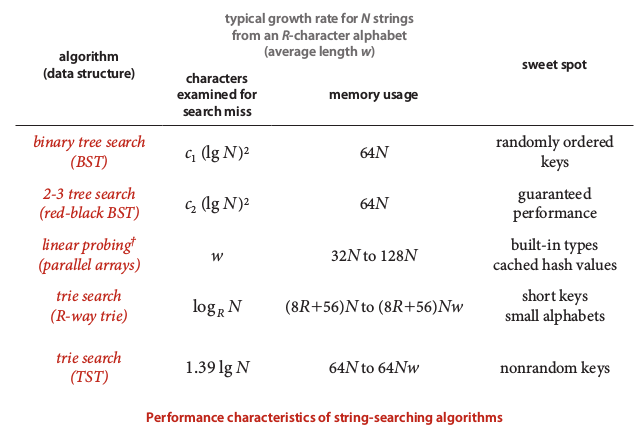
\includegraphics[width=.75\linewidth]{img/perf.png}
\label{perf}
\end{figure}

\subsection{Substring search}
\begin{myprob}[Substring search]
Given a \textit{text} string of length $N$ and
a pattern string of length $M$, find an occurence
of the pattern within the text.
\end{myprob}

\subsubsection{Rabin-Karp fingerprint search}
The Rabin-Karp algorithm uses hashing to solve this problem.
It's almost as simple as the brute-force algorithm but
runs in time proportional to $M+N$ with very high probability.
Furthermore, this algorithm extends to two-dimensional patterns,
which makes it more useful than the others for image processing.

\paragraph{Basic idea}
The basic idea behind this algorithm is the following: we compute
a hash function for the pattern and then look for a match by using
the same hash function for each possible $M$-character substring
of the text. If we find a text substring with the same hash value
as the pattern, we can check for a match.

\paragraph{Key idea}
A straightforward implementation based on this description would be much
slower than a brute-force search (since computing a hash function that involves
every character is likely to be much more expensive than just
comparing characters). But Rabin and Karp showed that it is easy
to compute hash functions for $M$-character substrings in
constant time, which leads to a linear-time substring search.

Using the notation $t_i$ for \lstinline|txt.charAt(i)|, the number
corresponding to the $M$-character substring of \lstinline|txt| that
starts at position \lstinline|i| using Horner's method is

\[ x_i = t_iR^{M-1} + t_{i+1}R^{M-2} + \dots + t_{i+M-1}R^0 \]

and we can assume that we know the value of $h(x_i) = x_i\bmod Q$.
Shifting one position right in the text corresponds to replacing
$x_i$ by

\[ x_{i+1} = (x_i - t_iR^{M-1})R + t_{i+M}. \]

We substract off the leading digit, multiply it by $R$, then add
the trailing digit. Now, the crucial point is that we do not have
to maintain the values of the numbers (i.e. $x_i$), just the
values of their remainders when divided by $Q$ (i.e. $h(x_i)$).
Remember the property of the modulus operation discussed in remark
\ref{rem:mod-prop}.

\paragraph{Implementation}
Here is the implementation of the \textit{Monte Carlo}
version of the Rabin-Karp fingerprint substring search.

\begin{mydef}[Monte Carlo and Las Vegas algorithms]
A \textit{Monte Carlo} algorithm is a randomized algorithm
whose running time is deterministic, but whose output may be
incorrect with a certain probability. On the other side, a
\textit{Las Vegas} algorithm is a randomized algorithm that
always gives correct results.
\end{mydef}

\lstinputlisting{code/RabinKarp.java}

\begin{myrem}
An extra \lstinline|Q| is added on line 36 to make sure that
everything is positive so that the remainder operation works as
it should.
\end{myrem}

By choosing a value of \lstinline|Q| greater than $10^{20}$, we
reduce the risk of collision, and thus reduce the probability
of the Monte Carlo algorithm failing. The alternative method
of checking for a match could be slow but is guaranteed correct.

\subsection{Data compression}
\begin{myprob}[Lossless compression]
The objective of data compression is to obtain two black boxes :
\begin{itemize}
	\item a \textit{compress} box that transforms a bitstream $B$
	into a compressed version $C(B)$;
	\item an \textit{expand} box that transforms $C(B)$ back into $B$.
\end{itemize}
Using the notation $\lvert B \rvert$ to denote the number of bits in the
bitstream, we are interested in minimizing the quantity $\lvert C(B)
\rvert/\lvert B \rvert$, which is known as the compression ratio.
\end{myprob}

\begin{mypropo}
Universal data compression is impossible, that is, no algorithm
can compress every bitstream.
\end{mypropo}

\subsubsection{Huffman compression}
The idea is to abandon the way in which text files are
usually stored: instead of using the usual 7 or 8 bits
for each character, we use fewer bits for characters that
appear often than for those that appear rarely.

A \textit{code} associates each character with a bitstring:
a symbol table with characters as keys and bitstrings as values.

Then, we take advantage of the fact that \textit{delimiters
are not needed if no character code is is the prefix of
another}. A code with this property is known as \textit{prefix
-free code}. All prefix-free codes are \textit{uniquely decodable}
(without needing any delimiters).

One convenient way to represent a prefix-free code is with
a trie. The general method for finding the optimal prefix-free
code is the hearth of Huffman compression.

\paragraph{Overview}
To compress a bitstream:
\begin{itemize}
	\item read the input;
	\item tabulate the frequency of occurrence of each
	\lstinline$char$ value in the input;
	\item build the Huffman encoding trie corresponding to
	those frequencies;
	\item build the corresponding codeword table to associate
	a bitstring with each \lstinline|char| value in the input;
	\item write the trie, encoded as bitstring;
	\item write the count of characters in the input, encoded
	as a bitstring;
	\item use the codeword table to write the codeword for each
	input character.
\end{itemize}

To expand a bitstream:
\begin{itemize}
	\item read the trie (encoded at the beginning of the bistream;
	\item read the count of characters to be decoded;
	\item use the trie to decode the bitstream.
\end{itemize}

\section{Graphs}

\subsection{Undirected graph}

\begin{mydef}[Graph]
A graph is a set of vertices and a collection of edges that each connect a
pair of vertices.
\end{mydef}

\paragraph{Anomalies}
Our definition allows two simple anomalies:
\begin{itemize}

\item a self-loop is an edge that connects a vertex to itself;
\item two edges that connect the same pair of vertices are parallel.

\end{itemize}

\begin{mydef}[Path]
A path in a graph is a sequence of vertices
connected by edges.
\end{mydef}
\begin{mydef}[Simple path]
A simple path is one with no repeated vertices.
\end{mydef}
\begin{mydef}[Cycle]
A cycle is a path with at least one edge whose first
and last vertices are the same.
\end{mydef}
\begin{mydef}[Simple cycle]
A simple cycle is a cycle with no repeated edges or vertices (except the
requisite repetition of the first and last vertices).
\end{mydef}
\begin{mydef}[Length]
The length of a path or a cycle is its number of edges.
\end{mydef}

\begin{mydef}[Connected graph]
A graph is connected if there is a path from every vertex to every other
vertex in the graph. A graph that is not connected consists of a set of
connected components, which are maximal connected subgraphs.
\end{mydef}
\begin{mydef}[Acyclic graph]
An acyclic graph is a graph with no cycles.
\end{mydef}
\begin{mydef}[Tree]
A tree is an acyclic connected graph.
\end{mydef}
\begin{mydef}[Forest]
A forest is a disjoint set of trees.
\end{mydef}
\begin{mydef}[Spanning tree]
A spanning tree of a connected graph is a subgraph that contains all of that
graph’s vertices and is a single tree. A spanning forest of
a graph is the union of spanning trees of its connected
components.
\end{mydef}

For example, a graph $G$ with $V$ vertices is a tree if and
only if it satisfies any of the following five conditions:

\begin{itemize}
\item $G$ has $V-1$ edges and no cycles;
\item $G$ has $V-1$ edges and is connected;
\item $G$ is connected, but removing any edge disconnects it;
\item $G$ is acyclic, but adding any edge creates a cycle;
\item exactly one simple path connects each pair of vertices in $G$.
\end{itemize}

\begin{mydef}[Bipartite graph]
A bipartite graph is a graph whose vertices we can divide into two sets
such that all edges connect a vertex in one set with a vertex in the other
set. An example of a bipartite graph is given in \figuref{bipart}, where one
set of vertices is colored red and the other set of vertices is colored black.
\end{mydef}

\begin{figure}[H]
	\centering
	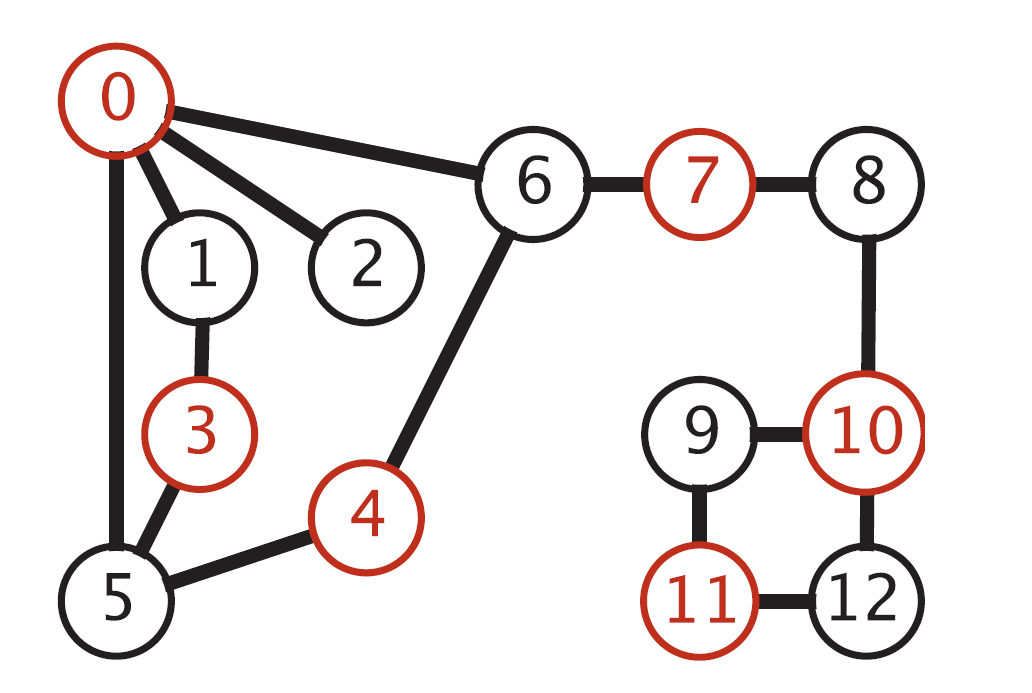
\includegraphics[scale=0.15]{img/graph_bipart.png}
	\caption{A bipartite graph.}
	\label{fig:bipart}
\end{figure}

\subsubsection{Different types of graph representations}

Different data structures exist:
\begin{itemize}
\item an incidence matrix;
\item an adjacency matrix;
\item an adjacency list.
\end{itemize}

\lstinline$adj(int v)$ is a method that allows iterating through the vertices
adjacent to a vertex \lstinline$v$.

The complexities of \lstinline$adj(int v)$ and
\lstinline$addEdge(int v, int w)$ are as follows:

\vspace{0.3cm}
\begin{tabular}{c|ccc}
& \textbf{Incidence matrix} & \textbf{Adjacency matrix} & \textbf{Adjacency
list}\\
\hline
\lstinline$adj(int v)$ & $\bigoh(\lvert E \rvert)$ & $\bigoh(1)$ &
$\bigoh(\lvert V \rvert)$\\
\lstinline$addEdge(int v, int w)$ & $\bigoh(\lvert V \rvert \cdot \lvert E
\rvert)$ & $\bigoh(1)$ & $\bigoh(1)$\\
\end{tabular}

\subsubsection{Undirected graph data type}
The undirected graph data type is made of three important local variables: an
integer variable \lstinline$V$ for the number of vertices, an integer variable
\lstinline$E$ for the number of edges and last but not least: an adjacency list
represented by a \lstinline$Bag<Integer>[]$ array.

\subsubsection{Depth-first search (DFS)}
The classic recursive method for searching in a connected graph (visiting all
of its vertices and edges) mimics Tr\'emaux's algorithm but is even simpler to
describe. To search a graph, invoke a recursive method that visits vertices. To
visit a vertex:
	\begin{itemize}
		\item mark it as having been visited;
		\item visit (recursively) all the vertices that are adjacent to it
		and have not yet been marked.
	\end{itemize}

The DFS algorithm below maintains an array of \lstinline$boolean$ values to
mark all of the vertices that are connected to the source (variable
\lstinline$s$).

\lstinputlisting{code/DepthFirstSearch.java}

\subsubsection{Depth-first path}

This \lstinline$Graph$ client uses depth-first search to find paths to all the
vertices in a graph that are connected to a given start vertex \lstinline$s$.
You will notice that the major part of this code is from the DFS.

\lstinputlisting{code/DepthFirstPath.java}

\begin{figure}[H]
	\centering
	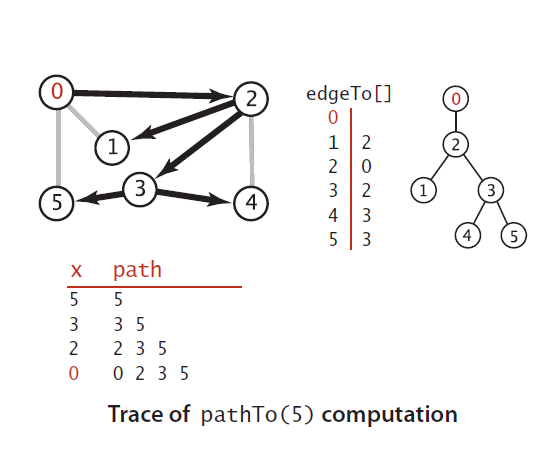
\includegraphics[scale=0.5]{img/dfp.png}
	\caption{Trace of \lstinline$pathTo(5)$ computation.}
	\label{fig:dfp}
\end{figure}

\subsection{Directed graph}

\begin{mydef}[Directed graph]
A directed graph (or digraph) is a set of vertices and a collection of directed
edges. Each directed edge connects an ordered pair of vertices.
\end{mydef}

\begin{mydef}[Directed path]
A directed path in a digraph is a sequence of vertices in which there is a
(directed) edge pointing from each vertex in the sequence to its successor in
the sequence.
\end{mydef}
\begin{mydef}[Directed cycle]
A directed cycle is a directed path with at least one edge whose first and last
vertices are the same.
\end{mydef}

\subsubsection{Directed DFS}

\lstinputlisting{code/DirectedDFS.java}
\paragraph{Note}
The \lstinline$!marked[s]$ condition in the \lstinline$DirectedDFS$ constructor
is useless since the \lstinline$boolean$ array was created just before and thus
all its entries are set to false\dots

\subsubsection{Directed cycle}

\begin{mydef}[Directed acyclic graph (DAG)]
A directed acyclic graph (DAG) is a digraph with no directed cycles.
\end{mydef}

This class adds to our standard recursive \lstinline$dfs()$ a
\lstinline$boolean$ array \lstinline$onStack[]$ to keep track of the vertices
for which the recursive call has not completed. When it finds an edge
\lstinline$v-w$ to a vertex \lstinline$w$ that is on the stack, it has
discovered a directed cycle, which it can recover by following
\lstinline$edgeTo[]$ links.

\lstinputlisting{code/DirectedCycle.java}

\begin{figure}[H]
	\centering
	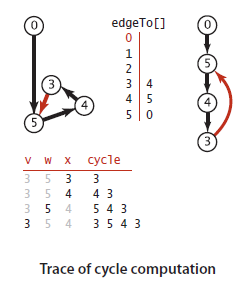
\includegraphics[scale=0.8]{img/directed_cycle.png}
	\caption{Trace of cycle computation.}
	\label{fig:directed cycle}
\end{figure}

\subsubsection{Topological sort}

\begin{mypropo}
A digraph has a topological order if and only if it is a DAG.
\end{mypropo}

Three vertex orderings are of interest in typical applications:

\begin{itemize}
\item preorder : put the vertex on a queue before the recursive calls;
\item postorder : put the vertex on a queue after the recursive calls;
\item reverse postorder : put the vertex on a stack after the recursive calls.
\end{itemize}

\begin{figure}[H]
	\centering
	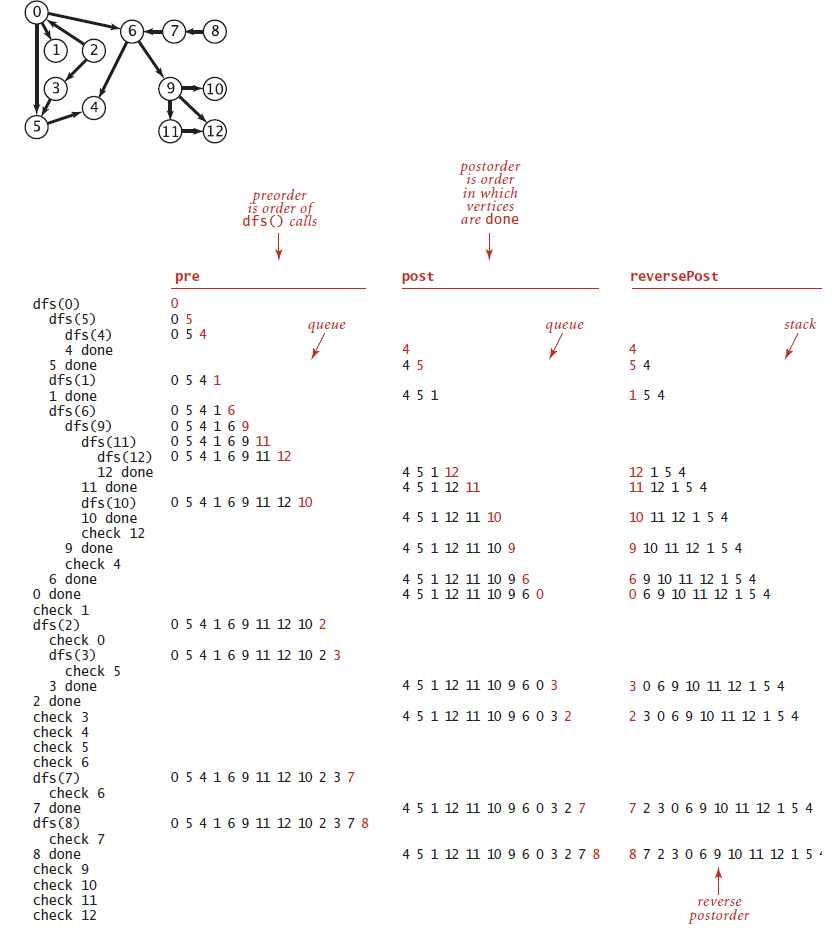
\includegraphics[width=\textwidth]{img/pre_post_rev.png}
	\caption{Computing depth-first orders in a digraph.}
	\label{fig:dfs_digraph}
\end{figure}

A one-line addition to our standard recursive DFS does the job! To convince
yourself of this fact, begin with the class \lstinline$DepthFirstOrder$

\lstinputlisting{code/DFSOrder.java}

\lstinputlisting{code/TopologicalSort.java}

\subsection{Minimum Spanning Tree}

\begin{mydef}[Edge-weighted graph]
With each edge $e$ of $G$ let there be associated a real number $w(e)$, called
its weight. Then $G$, together with these weights on its edges, is called an
edge-weighted graph (or a weighted graph).
\end{mydef}

\begin{mydef}[Minimum Spanning Tree (MST)]
A minimum spanning tree (MST) of an
edge-weighted graph is a spanning tree whose weight
(the sum of the weights of its edges) is no larger than
the weight of any other spanning tree.
\end{mydef}

\begin{mydef}[Cut]
A cut of a graph is a partition of its vertices into two nonempty disjoint
sets. A crossing edge of a cut is an edge that connects a vertex in one set
with a vertex in the other.
\end{mydef}

\paragraph{Edge-weighted graph data type}

\begin{figure}[H]
	\centering
	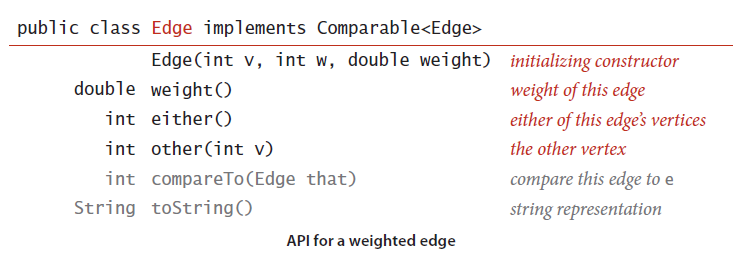
\includegraphics[scale=0.7]{img/edge_w_api.png}
	\label{fig:edge w api}
\end{figure}

\begin{mypropo}
Given any cut in an edge-weighted
graph, the crossing edge of minimum weight is in
the MST of the graph.
\end{mypropo}

\subsubsection{Prim's algorithm}

Prim's algorithm computes the MST of any connected edge-weighted graph.

\lstinputlisting{code/LazyPrimMST.java}

\subsubsection{Kruskal's algorithm}

\lstinputlisting{code/Kruskal2.java}

\subsubsection{Summary}

\begin{figure}[H]
	\centering
	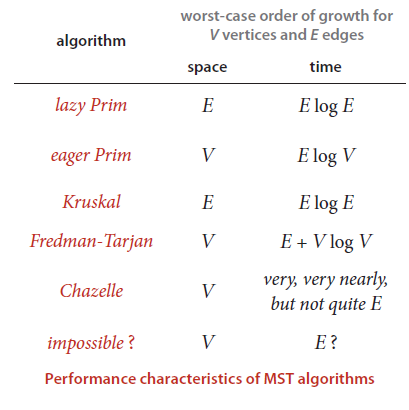
\includegraphics[scale=0.8]{img/summary_mst.png}
	\label{fig:summary MST}
\end{figure}

\begin{myrem}
Kruskal's algorithm is generally slower than Prim's algorithm because it has to
do a \lstinline$connected()$ operation for each edge, in addition to the
priority-queue operations that both algorithms do for each edge processed.
\end{myrem}

\subsection{Shortest path}

\begin{figure}[H]
	\centering
	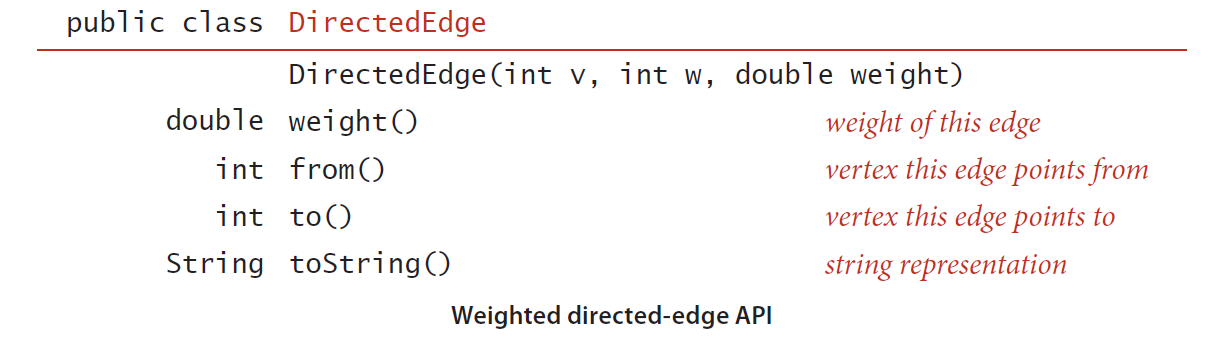
\includegraphics[scale=0.5]{img/directed_edge_w_api.png}
	\label{fig:directed w edge api}
\end{figure}


\subsubsection{Dijkstra's algorithm}
\lstinputlisting{code/Dijkstra.java}

\subsubsection{Summary}

\begin{figure}[H]
	\centering
	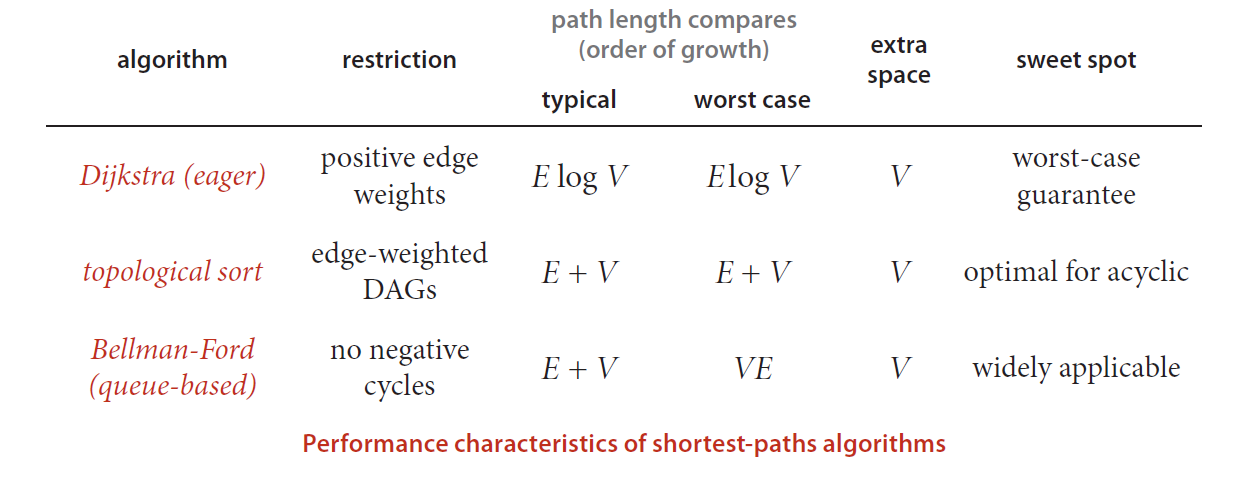
\includegraphics[scale=0.5]{img/summary_SPT.png}
	\label{fig:summary spt}
\end{figure}

% Need a better title for this section
\section{Various algorithms}
\subsection{Union-find}
\begin{mydef}[Union-find data structure]
A \textit{union-find} data structure is a data structure
that keeps track of a set of elements partitioned into
a number of disjoint subsets (equivalence classes).
\end{mydef}

The API is given in \figuref{uf-api}.

\begin{figure}[ht]
	\centering
	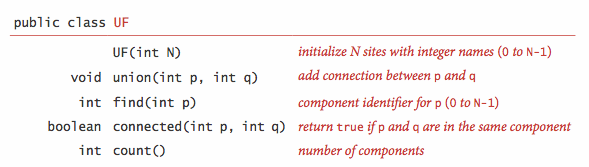
\includegraphics[scale=0.6]{img/uf-api.png}
	\caption{API of union-find data structure.}
	\label{fig:uf-api}
\end{figure}

This data structure helps to solve the \textit{dynamic
connectivity} problem. This problem arises for example
in networks. We will use networking terminology here.
We refer to the objects as \textit{sites}, the pairs
as \textit{connections} and the equivalence classes as
\textit{connected components} or \textit{components}.

When studying algorithms to implement the union-find API,
we count array accesses (the number of times an array entry
is accessed, for \emph{read} or \emph{write}).

We will consider three different implementations, all based
on using a site-indexed \lstinline|id[]| array.

\subsubsection{Quick-find}
Here we maintain the invariant that \lstinline|p| and
\lstinline|q| are connected if and only if \lstinline|id[p]|
is equal to \lstinline|id[q]|. Implementation is quite
straightforward. An overview of quick-find is given
in \figuref{quick-find-overview}.

\lstinputlisting{code/UnionFind.java}

\begin{myrem}
Note that here we made the arbitrary choice of
renaming the component containing \lstinline|p|.
\end{myrem}

\begin{mypropo}
The quick-find algorithm uses one array access for
each call to \lstinline|find()|, two array accesses
for each call to \lstinline|connected()| and
between $N+3$ and $2N+1$ array accesses for
each call to \lstinline|union()| that combines
two components.
\end{mypropo}

\begin{figure}[ht]
	\centering
	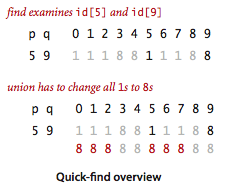
\includegraphics[scale=0.6]{img/quick-find-overview.png}
	\caption{Quick-find overview.}
	\label{fig:quick-find-overview}
\end{figure}

\subsubsection{Quick-union}
Here, the \lstinline|id[i]| entry for each site
is the name of another site in the same component
(possibly itself, in this case we call it a
\textit{root}) - we refer to this connection as a
\textit{link}. To implement \lstinline|find()|,
we start at the given site, follow its link to
another site, follow that site's link to yet
another site and so forth until reaching a root.
An overview of quick-union is given
in \figuref{quick-union-overview}.

\lstinputlisting{code/Find.java}

Two sites are in the same component if and
only if this process leads them to the same
root.

\lstinputlisting{code/Union.java}

\begin{figure}[ht]
	\centering
	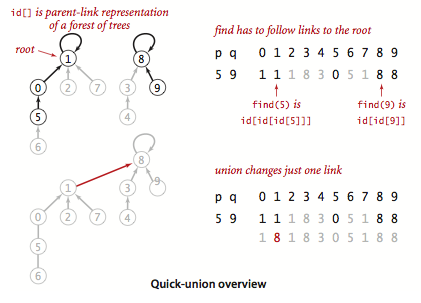
\includegraphics[scale=0.55]{img/quick-union-overview.png}
	\caption{Quick-union overview.}
	\label{fig:quick-union-overview}
\end{figure}

In \figuref{quick-union-overview}, we use the
\textit{forest-of-trees} representation. With this
representation, we can define some terminology.

\begin{mydef}{Size}
The \textit{size} of a tree is its number of nodes.
\end{mydef}
\begin{mydef}{Depth}
The \textit{depth} of a node in a tree is the number of links on the
path from it to the root.
\end{mydef}
\begin{mydef}{Height}
The \textit{height} of a tree is the maximum depth among its nodes.
\end{mydef}

\begin{mypropo}
The number of array accesses used by \lstinline|find()| in
quick-union is 1 plus twice the depth of the node corresponding
to the given site. The number of array accesses used by
\lstinline|union()| and \lstinline|connected()| is the cost
of the two \lstinline|find()| operations (plus 1 for \lstinline|union()|
if the given sites are in different trees).
\end{mypropo}

\subsubsection{Weighted quick-union}
Weighted quick-union is an improvement to quick-union algorithms
that allow us to reduce the tree height, and thus to reduce the
complexity of \lstinline|find()|.

\lstinputlisting{code/WeightedQuickUnion.java}

\begin{mypropo}
The depth of any node in a forest built by weighted
quick-union for $N$ sites is at most $\lg N$.
\end{mypropo}

\begin{mycorr}
For weighted quick-union with $N$ sites, the worst
case order of growth of the cost of \lstinline|find()|,
\lstinline|connected()| and \lstinline|union()| is
$\lg N$.
\end{mycorr}

\subsubsection{Summary}

\begin{table}[ht]
	\centering
	\begin{tabular}{c|ccc}
		\textbf{Algorithm} & \textbf{Constructor} & \textbf{Union} & \textbf{Find} \\
		\hline
		Quick-find & $N$ & $N$ & 1 \\
		Quick-union & $N$ & tree height & tree height \\
		Weigthed quick-union & $N$ & $\lg N$ & $\lg N$
	\end{tabular}
	\caption{Performance characteristics of union-find algorithms.}
	\label{tab:perf-uf}
\end{table}

\subsection{Priority queues}
A priority queue is an abstract data type with the API given
in \figuref{pq-api}. In this subsection, we will
consider a \lstinline|MaxPQ|. \lstinline|MinPQ| is easily
obtained from \lstinline|MaxPQ| (you only need to use
min-heap instead of a max-heap in what follows).

\begin{figure}[ht]
	\centering
	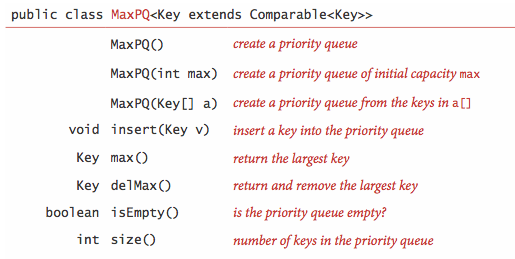
\includegraphics[scale=0.55]{img/pq-api.png}
	\caption{API of a priority queue.}
	\label{fig:pq-api}
\end{figure}

\subsubsection{Basic implementations}
Basic implementations using (un)ordered arrays or linked
list have the property that either the insert of the remove
maximum operation takes linear time in the worst case.

\subsubsection{Heap}
The binary heap is a data structure that can efficiently support
the basic priority queues operations. In a binary heap, the keys
are stored in an array such that each key is guaranteed to be
larger than (or equal to) the keys at two
other specific positions.

\begin{mydef}[Heap-ordered binary tree]
A binary tree is \textit{heap-ordered} if the key in each
node is larger than or equal to the keys in that node's
two children (if any).
\end{mydef}

\begin{mypropo}
The largest key in a heap-ordered binary tree is found at
the root.
\end{mypropo}

\begin{mydef}[Complete binary tree]
In a complete binary tree, every level, except possibly the
last, is completely filled, and all nodes in the last level
are as far left as possible.
\end{mydef}

A heap-ordered complete binary tree is illustrated in \figuref{heap}.

\begin{figure}[ht]
	\centering
	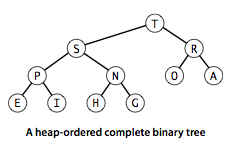
\includegraphics[scale=0.55]{img/heap.png}
	\caption{A heap-ordered complete binary tree.}
	\label{fig:heap}
\end{figure}

Complete trees provide the opportunity to use a compact
array representation (instead of explicit links as
for trees of \sectionref{tree}).

\begin{mydef}[Binary heap]
A binary heap is a collection of keys arranged in a complete
heap-ordered binary tree, represented in level order in an
array (not using the first entry).
\end{mydef}

In a heap, the parent of the node in position $k$ is in
position $\lfloor \frac{k}{2} \rfloor$ and, conversely,
the two children of the node in position $k$ are in
positions $2k$ and $2k+1$. This allows us to travel
up and down the tree simply by doing arithmetic
on array indices.

\begin{mypropo}
The height of a complete binary tree of size $N$ is
$\lfloor \lg N \rfloor$
\end{mypropo}

\paragraph{Heap algorithms}
Operations on heaps could violate the heap condition.
The process of restoring the heap order is called
\textit{reheapifying}. There are two types of violations
and thus two algorithms to reheapify.

\subparagraph{Bottom-up reheapify (swim)}
If the heap order is violated because a node's key becomes
larger than that node's parent's key, then we can make
progress toward fixing the violation by exchanging the node
with its parent (and so forth, moving up until we reach a
node with a larger key, or the root) as can be seen in \figuref{swim}.

\lstinputlisting{code/Swim.java}

\subparagraph{Top-down reheapify (sink)}
If the heap order is violated because a node's key
becomes smaller than one or both of that node's children's
keys, then we can make progress toward fixing the
violation by exchanging the node with the larger
of its two children (and so forth, moving down until
we reach a node with both children smaller (or equal),
or the bottom) as can be seen in \figuref{sink}.

\lstinputlisting{code/Sink.java}

\begin{figure}[ht]
	\centering
	\begin{subfigure}{.5\textwidth}
		\centering
  		\includegraphics[width=.85\linewidth]{img/swim.png}
 		\caption{Swim.}
  		\label{fig:swim}
	\end{subfigure}%
	\begin{subfigure}{.5\textwidth}
  		\centering
  		\includegraphics[width=0.73\linewidth]{img/sink.png}
  		\caption{Sink.}
  		\label{fig:sink}
	\end{subfigure}
	\caption{}
	\label{fig:reheap}
\end{figure}

\paragraph{Implementations}
Now that we can reheapify, implementing \lstinline|MaxPQ|
is quite straightforward.

\lstinputlisting{code/MaxPQ.java}

Heap operations are illustrated in \figuref{heap-ops}.

\begin{figure}[ht]
	\centering
	\includegraphics[scale=0.55]{img/heap-ops.png}
	\caption{Heap operations.}
	\label{fig:heap-ops}
\end{figure}

\begin{mypropo}
In an $N$-item priority queue, the heap algorithms
require no more than $1 + \lg N$ compares for
\emph{insert} and no more than $2\lg N$ compares
for \emph{remove the maximum}.
\end{mypropo}

\end{document}
